\chapter{Eksploratorna analiza}

\section{Opis atributa}
opis atributa....

\section{Vizualizacija Podataka}
	Vizualizacija podataka postaje ključna komponenta analize i interpretacije kompleksnih skupova podataka. 
	U ovom podpoglavlju istražujemo moć vizualizacije u kontekstu glazbene platforme Spotify, prezentirajući neke od grafova kako bismo bolje razumjeli glazbene obrasce, preferencije slušatelja te dinamiku glazbene industrije.
	
	\subsubsection{1) Top 10 Artists Based on Popularity}
	
	\textbf{Opis grafa:}
	
	Ovaj graf prikazuje deset najpopularnijih glazbenih izvođača temeljem prosječne popularnosti njihovih pjesama. Izračunata je srednja vrijednost popularnosti za svakog izvođača, a zatim su odabrani najbolji deset izvođača prema toj mjeri popularnosti.
	
	Na x-osi su navedeni izvođači, poredani prema visini prosječne popularnosti, dok y-os prikazuje prosječnu popularnost. Svaki šareni stupac predstavlja jednog izvođača, a visina stupa označava njegovu prosječnu popularnost.
	
	Ovaj graf pruža brz i pregledan način usporedbe popularnosti izvođača, omogućujući identifikaciju najboljih deset temeljem prosjeka popularnosti njihovih pjesama.
	
	\textbf{Slika grafa:}
	\begin{figure}[H]
		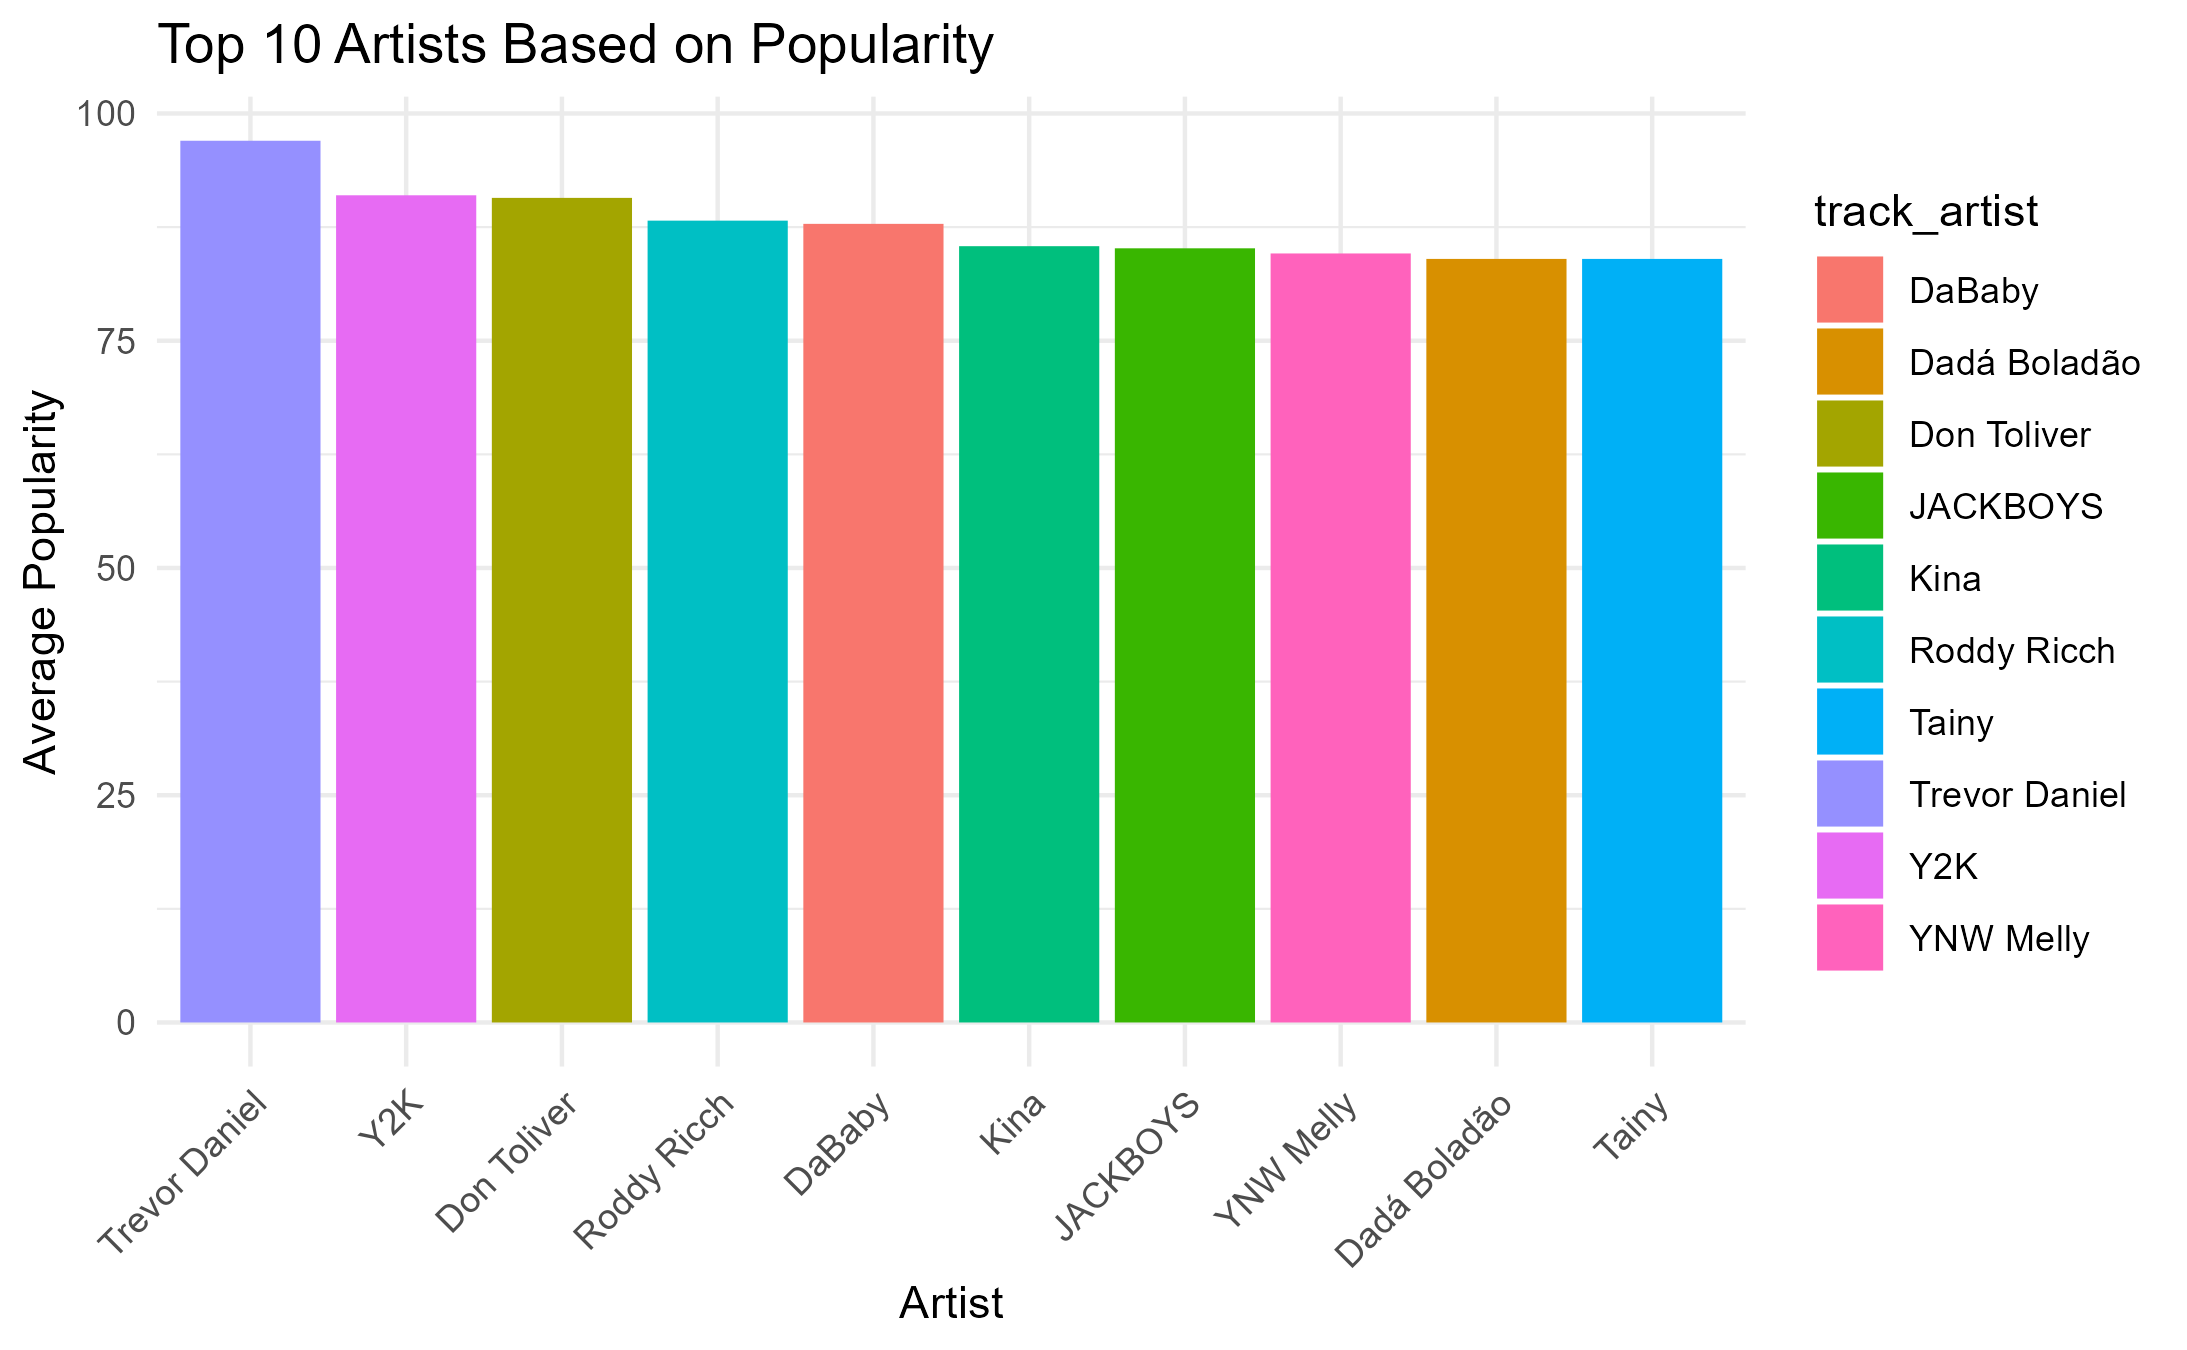
\includegraphics[scale=0.9]{slike/Top 10 popularity}
		%veličina slike u odnosu na originalnu datoteku i pozicija slike
		\centering
		\caption{Top 10 Artists Based on Popularity}
		
	\end{figure}

\eject



